\documentclass[]{beamer}
%language
\usepackage[ngerman,english]{babel}
\usepackage[utf8]{inputenc}
\usepackage{xspace}
\usepackage{amsmath,amssymb}
\usepackage{ulem}

\usepackage{algpseudocode}
\usepackage{listings}

\usepackage{tikz}
\usetikzlibrary{mindmap}

\usepackage[utf8]{inputenc}
%theme
\useoutertheme[nofootline]{wuerzburg}
\useinnertheme{chamfered}
\usecolortheme{shark}

%title setup
\title{Generischer Titel: Studie - Emailkryptographie}
%\subtitle{Montag 12-14, Raum 01.150-128}
\subtitle{Human Factors in IT-Security}
\author{Ulrich Dorsch, Tim Grocki, Leonhard Hösch  \\ {\tiny ulrichdorsch@googlemail.com, tgrocki@lavabit.com, lh@dancingwolf.de \\}}
\institute[Universität Erlangen]{Friedrich-Alexander-Universität Erlangen
\\Department Informatik \\ Lehrstuhl 1}


\AtBeginSection[]
{
	\begin{frame}
		\frametitle{Überblick}
		\tiny{\tableofcontents[currentsection]}
	\end{frame}
}

\begin{document}
%titlepage
\begin{frame}
	\titlepage
\end{frame}


\begin{frame}
	\begin{center}
		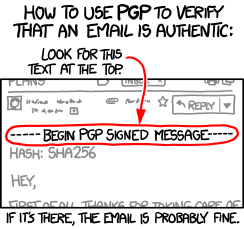
\includegraphics[scale=0.7]{pic/pgp.png}\phantom{\footnote{\url{http://xkcd.com/1181/}}}
	\end{center}

\end{frame}

\section{Überblick}

\subsection{Motivation}
\begin{frame}{Motivation}
\begin{itemize}
	\item Emailkryptographie ist nicht weit verbreitet, obwohl es viele Gründe für dessen Einsatz gibt.
	\item Studien haben versucht zu zeigen, dass schlechte Usability der Grund für die geringe Verbreitung ist.
	\item Wir haben uns bemüht, dies mit unserer Studie zu überprüfen.
\end{itemize}
\end{frame}


\subsection{Forschungsfrage}
\begin{frame}{Forschungsfrage}
	Sind Usability Probleme tatsächlich die Hauptgründe für die geringe Verbreitung von Email\-kryp\-to\-gra\-phie?

	Welche anderen Ursachen spielen eine (wie große) Rolle?
\end{frame}

\subsection{Hypothese}
\begin{frame}{Hypothese}
	Usability ist nicht das primäre Problem, da mehr als 50\% der
	potenziellen Nutzer durch andere Ursachen davon abgehalten werden,
	Email\-kryp\-to\-gra\-phie einzusetzen.
\begin{block}{Usability Problem - Definition}
	In unserem Kontext betrachten wir ein Usability Problem als eine technische Hürde,
	die die Benutzung von Emailkryptographie verhindert oder deutlich erschwert.
\end{block}
\end{frame}

\section{Umfrageumstände}
%% NSA
\begin{frame}{NSA Skandal}
	bla
\end{frame}

\section{Demographische Daten}
\begin{frame}{Demographische Daten}
	\begin{center}
		Studienfächer
	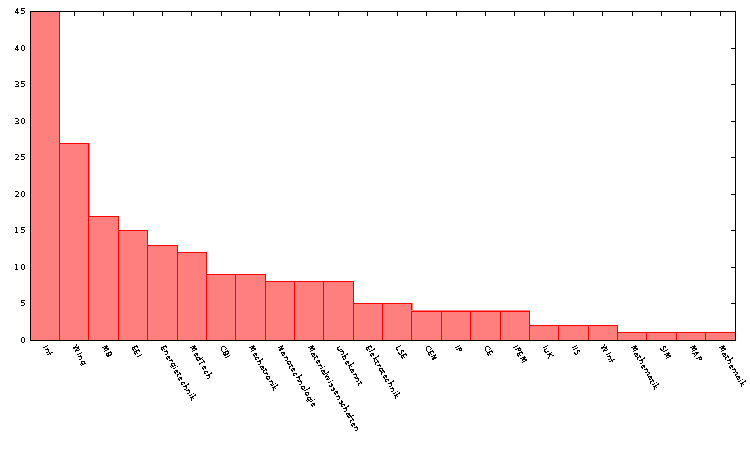
\includegraphics[scale=0.9]{plots/stud.pdf}
	\end{center}
\end{frame}

\section{Auswertung der Antworten}
\subsection{Interesse an Emailkryptographie}
\begin{frame}{Interesse an Emailkryptographie}
	
\end{frame}

\subsection{Bekanntheit von Gefahren}
\begin{frame}{Bekanntheit von Gefahren}
	
\end{frame}

\subsection{Schema des Fragebogens}
\begin{frame}{Fragebogenverlauf}
	\begin{tikzpicture}[mindmap,scale=0.7]
		\path[concept color=blue,every concept/.append style={scale=0.7}]
		node[concept] {255 \\ 100\%}
			child[concept color=blue,grow=-5] {node[concept] {N}}
			child[concept color=gray,grow=-170] {node[concept] {installiert}
				child[concept color=gray,grow=-30] {node[concept] {war inst.}
					child[concept color=gray,grow=-90] {node[concept] {delete}
						child[concept color=gray,grow=-130] {node[concept] {U}}
						child[concept color=gray,grow=-70] {node[concept] {U}}
					}
					child[concept color=gray,grow=-10] {node[concept] {geplant}
						child[concept color=gray,grow=0] {node[concept] {N}}
						child[concept color=gray,grow=-60] {node[concept] {versucht}
							child[concept color=gray,grow=-130] {node[concept] {U}}
							child[concept color=gray,grow=-50] {node[concept] {N}}
						}
					}
				}
				child[concept color=gray,grow=-130] {node[concept] {reglm}
					child[concept color=gray,grow=-130] {node[concept] {N}}
					child[concept color=gray,grow=-70] {node[concept] {jemals}
						child[concept color=gray,grow=-130] {node[concept] {U}}
						child[concept color=gray,grow=-70] {node[concept] {kontakt}
							child[concept color=gray,grow=-130] {node[concept] {U}}
							child[concept color=gray,grow=-70] {node[concept] {N}}
						}
					}
				}
			};
			\node[annotation,below,fill=gray!50,scale=1.3] at (4,-6.4) {some text goes here};
	\end{tikzpicture}
\end{frame}

\begin{frame}{Fragebogenverlauf}
	\begin{tikzpicture}[mindmap,scale=0.7]
		\path[concept color=blue,every concept/.append style={scale=0.7}]
		node[concept] {255 \\ 100\%}
			child[concept color=gray,grow=-5] {node[concept] {N}}
			child[concept color=blue,grow=-170] {node[concept] {installiert}
				child[concept color=gray,grow=-30] {node[concept] {war inst.}
					child[concept color=gray,grow=-90] {node[concept] {delete}
						child[concept color=gray,grow=-130] {node[concept] {U}}
						child[concept color=gray,grow=-70] {node[concept] {U}}
					}
					child[concept color=gray,grow=-10] {node[concept] {geplant}
						child[concept color=gray,grow=0] {node[concept] {N}}
						child[concept color=gray,grow=-60] {node[concept] {versucht}
							child[concept color=gray,grow=-130] {node[concept] {U}}
							child[concept color=gray,grow=-50] {node[concept] {N}}
						}
					}
				}
				child[concept color=blue,grow=-130] {node[concept] {reglm}
					child[concept color=blue,grow=-130] {node[concept] {N}}
					child[concept color=gray,grow=-70] {node[concept] {jemals}
						child[concept color=gray,grow=-130] {node[concept] {U}}
						child[concept color=gray,grow=-70] {node[concept] {kontakt}
							child[concept color=gray,grow=-130] {node[concept] {U}}
							child[concept color=gray,grow=-70] {node[concept] {N}}
						}
					}
				}
			};
			\node[annotation,below,fill=gray!50,scale=1.3] at (4,-6.4) {some text goes here};
	\end{tikzpicture}
\end{frame}


\begin{frame}{Fragebogenverlauf}
	\begin{tikzpicture}[mindmap,scale=0.7]
		\path[concept color=blue,every concept/.append style={scale=0.7}]
		node[concept] {255 \\ 100\%}
			child[concept color=gray,grow=-5] {node[concept] {N}}
			child[concept color=blue,grow=-170] {node[concept] {installiert}
				child[concept color=gray,grow=-30] {node[concept] {war inst.}
					child[concept color=gray,grow=-90] {node[concept] {delete}
						child[concept color=gray,grow=-130] {node[concept] {U}}
						child[concept color=gray,grow=-70] {node[concept] {U}}
					}
					child[concept color=gray,grow=-10] {node[concept] {geplant}
						child[concept color=gray,grow=0] {node[concept] {N}}
						child[concept color=gray,grow=-60] {node[concept] {versucht}
							child[concept color=gray,grow=-130] {node[concept] {U}}
							child[concept color=gray,grow=-50] {node[concept] {N}}
						}
					}
				}
				child[concept color=blue,grow=-130] {node[concept] {reglm}
					child[concept color=gray,grow=-130] {node[concept] {N}}
					child[concept color=blue,grow=-70] {node[concept] {jemals}
						child[concept color=blue,grow=-130] {node[concept] {U}}
						child[concept color=gray,grow=-70] {node[concept] {kontakt}
							child[concept color=gray,grow=-130] {node[concept] {U}}
							child[concept color=gray,grow=-70] {node[concept] {N}}
						}
					}
				}
			};
			\node[annotation,below,fill=gray!50,scale=1.3] at (4,-6.4) {some text goes here};
	\end{tikzpicture}
\end{frame}


\begin{frame}{Fragebogenverlauf}
	\begin{tikzpicture}[mindmap,scale=0.7]
		\path[concept color=blue,every concept/.append style={scale=0.7}]
		node[concept] {255 \\ 100\%}
			child[concept color=gray,grow=-5] {node[concept] {N}}
			child[concept color=blue,grow=-170] {node[concept] {installiert}
				child[concept color=gray,grow=-30] {node[concept] {war inst.}
					child[concept color=gray,grow=-90] {node[concept] {delete}
						child[concept color=gray,grow=-130] {node[concept] {U}}
						child[concept color=gray,grow=-70] {node[concept] {U}}
					}
					child[concept color=gray,grow=-10] {node[concept] {geplant}
						child[concept color=gray,grow=0] {node[concept] {N}}
						child[concept color=gray,grow=-60] {node[concept] {versucht}
							child[concept color=gray,grow=-130] {node[concept] {U}}
							child[concept color=gray,grow=-50] {node[concept] {N}}
						}
					}
				}
				child[concept color=blue,grow=-130] {node[concept] {reglm}
					child[concept color=gray,grow=-130] {node[concept] {N}}
					child[concept color=blue,grow=-70] {node[concept] {jemals}
						child[concept color=gray,grow=-130] {node[concept] {U}}
						child[concept color=blue,grow=-70] {node[concept] {kontakt}
							child[concept color=blue,grow=-130] {node[concept] {U}}
							child[concept color=gray,grow=-70] {node[concept] {N}}
						}
					}
				}
			};
			\node[annotation,below,fill=gray!50,scale=1.3] at (4,-6.4) {some text goes here};
	\end{tikzpicture}
\end{frame}

\begin{frame}{Fragebogenverlauf}
	\begin{tikzpicture}[mindmap,scale=0.7]
		\path[concept color=blue,every concept/.append style={scale=0.7}]
		node[concept] {255 \\ 100\%}
			child[concept color=gray,grow=-5] {node[concept] {N}}
			child[concept color=blue,grow=-170] {node[concept] {installiert}
				child[concept color=gray,grow=-30] {node[concept] {war inst.}
					child[concept color=gray,grow=-90] {node[concept] {delete}
						child[concept color=gray,grow=-130] {node[concept] {U}}
						child[concept color=gray,grow=-70] {node[concept] {U}}
					}
					child[concept color=gray,grow=-10] {node[concept] {geplant}
						child[concept color=gray,grow=0] {node[concept] {N}}
						child[concept color=gray,grow=-60] {node[concept] {versucht}
							child[concept color=gray,grow=-130] {node[concept] {U}}
							child[concept color=gray,grow=-50] {node[concept] {N}}
						}
					}
				}
				child[concept color=blue,grow=-130] {node[concept] {reglm}
					child[concept color=gray,grow=-130] {node[concept] {N}}
					child[concept color=blue,grow=-70] {node[concept] {jemals}
						child[concept color=gray,grow=-130] {node[concept] {U}}
						child[concept color=blue,grow=-70] {node[concept] {kontakt}
							child[concept color=gray,grow=-130] {node[concept] {U}}
							child[concept color=blue,grow=-70] {node[concept] {N}}
						}
					}
				}
			};
			\node[annotation,below,fill=gray!50,scale=1.3] at (4,-6.4) {some text goes here};
	\end{tikzpicture}
\end{frame}



\begin{frame}{Fragebogenverlauf}
	\begin{tikzpicture}[mindmap,scale=0.7]
		\path[concept color=blue,every concept/.append style={scale=0.7}]
		node[concept] {255 \\ 100\%}
			child[concept color=gray,grow=-5] {node[concept] {N}}
			child[concept color=blue,grow=-170] {node[concept] {installiert}
				child[concept color=blue,grow=-30] {node[concept] {war inst.}
					child[concept color=blue,grow=-90] {node[concept] {delete}
						child[concept color=blue,grow=-130] {node[concept] {U}}
						child[concept color=gray,grow=-70] {node[concept] {U}}
					}
					child[concept color=gray,grow=-10] {node[concept] {geplant}
						child[concept color=gray,grow=0] {node[concept] {N}}
						child[concept color=gray,grow=-60] {node[concept] {versucht}
							child[concept color=gray,grow=-130] {node[concept] {U}}
							child[concept color=gray,grow=-50] {node[concept] {N}}
						}
					}
				}
				child[concept color=gray,grow=-130] {node[concept] {reglm}
					child[concept color=gray,grow=-130] {node[concept] {N}}
					child[concept color=gray,grow=-70] {node[concept] {jemals}
						child[concept color=gray,grow=-130] {node[concept] {U}}
						child[concept color=gray,grow=-70] {node[concept] {kontakt}
							child[concept color=gray,grow=-130] {node[concept] {U}}
							child[concept color=gray,grow=-70] {node[concept] {N}}
						}
					}
				}
			};
			\node[annotation,below,fill=gray!50,scale=1.3] at (4,-6.4) {some text goes here};
	\end{tikzpicture}
\end{frame}


\begin{frame}{Fragebogenverlauf}
	\begin{tikzpicture}[mindmap,scale=0.7]
		\path[concept color=blue,every concept/.append style={scale=0.7}]
		node[concept] {255 \\ 100\%}
			child[concept color=gray,grow=-5] {node[concept] {N}}
			child[concept color=blue,grow=-170] {node[concept] {installiert}
				child[concept color=blue,grow=-30] {node[concept] {war inst.}
					child[concept color=blue,grow=-90] {node[concept] {delete}
						child[concept color=gray,grow=-130] {node[concept] {U}}
						child[concept color=blue,grow=-70] {node[concept] {U}}
					}
					child[concept color=gray,grow=-10] {node[concept] {geplant}
						child[concept color=gray,grow=0] {node[concept] {N}}
						child[concept color=gray,grow=-60] {node[concept] {versucht}
							child[concept color=gray,grow=-130] {node[concept] {U}}
							child[concept color=gray,grow=-50] {node[concept] {N}}
						}
					}
				}
				child[concept color=gray,grow=-130] {node[concept] {reglm}
					child[concept color=gray,grow=-130] {node[concept] {N}}
					child[concept color=gray,grow=-70] {node[concept] {jemals}
						child[concept color=gray,grow=-130] {node[concept] {U}}
						child[concept color=gray,grow=-70] {node[concept] {kontakt}
							child[concept color=gray,grow=-130] {node[concept] {U}}
							child[concept color=gray,grow=-70] {node[concept] {N}}
						}
					}
				}
			};
			\node[annotation,below,fill=gray!50,scale=1.3] at (4,-6.4) {some text goes here};
	\end{tikzpicture}
\end{frame}


\begin{frame}{Fragebogenverlauf}
	\begin{tikzpicture}[mindmap,scale=0.7]
		\path[concept color=blue,every concept/.append style={scale=0.7}]
		node[concept] {255 \\ 100\%}
			child[concept color=gray,grow=-5] {node[concept] {N}}
			child[concept color=blue,grow=-170] {node[concept] {installiert}
				child[concept color=blue,grow=-30] {node[concept] {war inst.}
					child[concept color=gray,grow=-90] {node[concept] {delete}
						child[concept color=gray,grow=-130] {node[concept] {U}}
						child[concept color=gray,grow=-70] {node[concept] {U}}
					}
					child[concept color=blue,grow=-10] {node[concept] {geplant}
						child[concept color=gray,grow=0] {node[concept] {N}}
						child[concept color=blue,grow=-60] {node[concept] {versucht}
							child[concept color=blue,grow=-130] {node[concept] {U}}
							child[concept color=gray,grow=-50] {node[concept] {N}}
						}
					}
				}
				child[concept color=gray,grow=-130] {node[concept] {reglm}
					child[concept color=gray,grow=-130] {node[concept] {N}}
					child[concept color=gray,grow=-70] {node[concept] {jemals}
						child[concept color=gray,grow=-130] {node[concept] {U}}
						child[concept color=gray,grow=-70] {node[concept] {kontakt}
							child[concept color=gray,grow=-130] {node[concept] {U}}
							child[concept color=gray,grow=-70] {node[concept] {N}}
						}
					}
				}
			};
			\node[annotation,below,fill=gray!50,scale=1.3] at (4,-6.4) {some text goes here};
	\end{tikzpicture}
\end{frame}


\begin{frame}{Fragebogenverlauf}
	\begin{tikzpicture}[mindmap,scale=0.7]
		\path[concept color=blue,every concept/.append style={scale=0.7}]
		node[concept] {255 \\ 100\%}
			child[concept color=gray,grow=-5] {node[concept] {N}}
			child[concept color=blue,grow=-170] {node[concept] {installiert}
				child[concept color=blue,grow=-30] {node[concept] {war inst.}
					child[concept color=gray,grow=-90] {node[concept] {delete}
						child[concept color=gray,grow=-130] {node[concept] {U}}
						child[concept color=gray,grow=-70] {node[concept] {U}}
					}
					child[concept color=blue,grow=-10] {node[concept] {geplant}
						child[concept color=gray,grow=0] {node[concept] {N}}
						child[concept color=blue,grow=-60] {node[concept] {versucht}
							child[concept color=gray,grow=-130] {node[concept] {U}}
							child[concept color=blue,grow=-50] {node[concept] {N}}
						}
					}
				}
				child[concept color=gray,grow=-130] {node[concept] {reglm}
					child[concept color=gray,grow=-130] {node[concept] {N}}
					child[concept color=gray,grow=-70] {node[concept] {jemals}
						child[concept color=gray,grow=-130] {node[concept] {U}}
						child[concept color=gray,grow=-70] {node[concept] {kontakt}
							child[concept color=gray,grow=-130] {node[concept] {U}}
							child[concept color=gray,grow=-70] {node[concept] {N}}
						}
					}
				}
			};
			\node[annotation,below,fill=gray!50,scale=1.3] at (4,-6.4) {some text goes here};
	\end{tikzpicture}
\end{frame}

\begin{frame}{Fragebogenverlauf}
	\begin{tikzpicture}[mindmap,scale=0.7]
		\path[concept color=blue,every concept/.append style={scale=0.7}]
		node[concept] {255 \\ 100\%}
			child[concept color=gray,grow=-5] {node[concept] {N}}
			child[concept color=blue,grow=-170] {node[concept] {installiert}
				child[concept color=blue,grow=-30] {node[concept] {war inst.}
					child[concept color=gray,grow=-90] {node[concept] {delete}
						child[concept color=gray,grow=-130] {node[concept] {U}}
						child[concept color=gray,grow=-70] {node[concept] {U}}
					}
					child[concept color=blue,grow=-10] {node[concept] {geplant}
						child[concept color=blue,grow=0] {node[concept] {N}}
						child[concept color=gray,grow=-60] {node[concept] {versucht}
							child[concept color=gray,grow=-130] {node[concept] {U}}
							child[concept color=gray,grow=-50] {node[concept] {N}}
						}
					}
				}
				child[concept color=gray,grow=-130] {node[concept] {reglm}
					child[concept color=gray,grow=-130] {node[concept] {N}}
					child[concept color=gray,grow=-70] {node[concept] {jemals}
						child[concept color=gray,grow=-130] {node[concept] {U}}
						child[concept color=gray,grow=-70] {node[concept] {kontakt}
							child[concept color=gray,grow=-130] {node[concept] {U}}
							child[concept color=gray,grow=-70] {node[concept] {N}}
						}
					}
				}
			};
			\node[annotation,below,fill=gray!50,scale=1.3] at (4,-6.4) {some text goes here};
	\end{tikzpicture}
\end{frame}



\subsection{Auswertung}
\begin{frame}{Auswertung}
	\begin{tikzpicture}[mindmap,scale=0.7]
		\path[concept color=gray,every concept/.append style={scale=0.7}]
		node[concept] {255 \\ 100\%}
			child[concept color=gray,grow=-5] {node[concept] {N}}
			child[concept color=gray,grow=-170] {node[concept] {installiert}
				child[concept color=gray,grow=-30] {node[concept] {war inst.}
					child[concept color=gray,grow=-90] {node[concept] {delete}
						child[concept color=gray,grow=-130] {node[concept] {U}}
						child[concept color=gray,grow=-70] {node[concept] {U}}
					}
					child[concept color=gray,grow=-10] {node[concept] {geplant}
						child[concept color=gray,grow=0] {node[concept] {N}}
						child[concept color=gray,grow=-60] {node[concept] {versucht}
							child[concept color=gray,grow=-130] {node[concept] {U}}
							child[concept color=gray,grow=-50] {node[concept] {N}}
						}
					}
				}
				child[concept color=gray,grow=-130] {node[concept] {reglm}
					child[concept color=gray,grow=-130] {node[concept] {N}}
					child[concept color=gray,grow=-70] {node[concept] {jemals}
						child[concept color=gray,grow=-130] {node[concept] {U}}
						child[concept color=gray,grow=-70] {node[concept] {kontakt}
							child[concept color=gray,grow=-130] {node[concept] {U}}
							child[concept color=gray,grow=-70] {node[concept] {N}}
						}
					}
				}
			};
	\end{tikzpicture}
\end{frame}
\subsection{Details}
% detailfragen
\begin{frame}{Details}
	
\end{frame}

\section{Forschungsergebnis}
\begin{frame}{Forschungsergebnis}
	
\end{frame}

\section{Einschränkungen}
% meta probleme
% problem: knappe frage Emailkryptographie <-> unbekanter begriff
% hauptsächlich techniker/studenten
\begin{frame}{Einschränkungen}
	
\end{frame}


\end{document}
